\documentclass[12pt,AutoFakeBold]{article} 

% 注意:本模板还是存在一定的问题的,指导老师评语和实验报告内容基本要求之间本不应该有空隙,但我不会处理,但这个小问题没有人管。

\usepackage[数字电路与逻辑设计实验]{XDULabreport}  % 载入 XDULabreport 模板文件,[]中填写科目名称,科目名称,默认为电子线路实验(I)
\problem{交通灯控制器}  % 请在此处填写问题内容
\coauthor{丁辉} % 同作者姓名
\labdate{2021年10月31日} % 实验日期
% 其他参数在宏包中进行更改,其中学院,班级,姓名,学号均在sty宏包内进行更改
% \usepackage{fourier}  % 这是 fourier 字体,更柔和 

\newfontfamily\digi{DigifaceWide Regular} % 将数码管字体引入

%% 如果你需要中文的一级标题编号,如“一、”、“二、”等,请把下面两行取消注释
% \RequirePackage{zhnumber} % change section number to chinese
% \titleformat{\section}{\Large\bfseries\rmfamily}{\zhnum{section}、}{0em}{}

% 文档开始
        
\begin{document}

\maketitle
\setcounter{tocdepth}{2}
\tableofcontents  % 生成目录

% 正文标题
\makeatletter
\begin{center}
	\LARGE \textbf{\textsf{\@problem}}
\end{center}
\makeatother


% 正文开始


\section{实验目的}

掌握基本的时序逻辑设计方法,学习利用计数器和状态机设计交通灯控制器。分两个方向 (1,2),每个方向各有红 (R)、绿 (G) 两个交通灯。按下按钮 $K0\sim K3$ 时直接进入对应序号的状态,随后即转入自动方式。在自动方式下,控制器的状态转移表如表 \ref{table:trans} 所示。


\begin{table}[hbtp]
	\setlength{\abovecaptionskip}{0cm} 
	\setlength{\belowcaptionskip}{-0.2cm}
	\begin{center}
	\caption{状态转移表}
	\begin{tabular}{|c|c|c|}
		\hline
		\textbf{状态} & \textbf{亮灯} & \textbf{停留时间} \\ \hline
		S0          & R1,G2       & 2s            \\ \hline
		S1          & R1          & 1s            \\ \hline
		S2          & G1,R2       & 2s            \\ \hline
		S3          & R2          & 1s            \\ \hline
	\end{tabular}\label{table:trans}
	\end{center}
\end{table}


\section{实验环境}

\begin{itemize}
	\item Quartus II 13.0: 创建项目,编写 Verilog HDL 代码,并进行编译之后生成 Test Bench 模板,输入信号进行仿真
	\item ModelSim ALTERA 10.4d: 进行仿真获得仿真波形
	\item \LaTeX: 制作封面并进行文档编写排版
	\item Visio 2016: 用于原理框图的绘制
\end{itemize}

\section{方案设计及理论计算}

方案设计分为三个模块,分别为分频器模块 (clk\_div)、按键防抖模块 (key\_scan)、红绿灯状态转换模块(led\_trans),它们之间的关系可用如图 \ref{fig:theory} 所示的原理框图表示

\begin{figure}[hbtp]
	\centering
	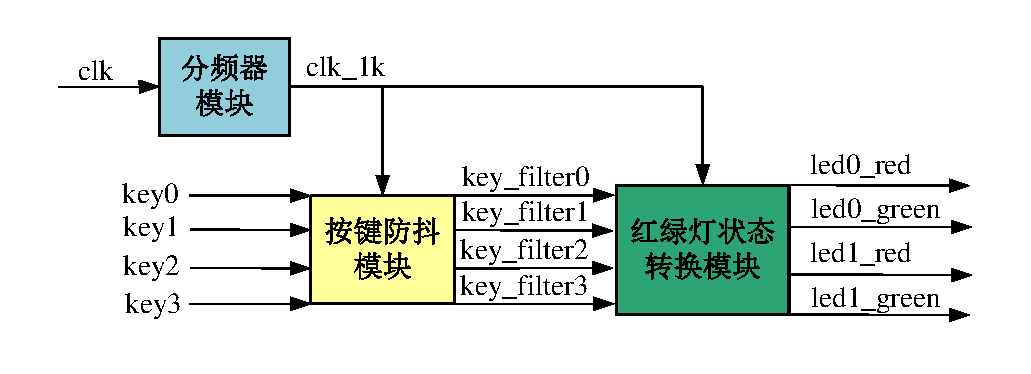
\includegraphics[width=16cm]{theory.pdf}
	\caption{原理框图}\label{fig:theory}
\end{figure}

\subsection{分频器模块}

在交通灯控制系统中,通过自动控制方式指挥交通。因此需要给电路一个稳定的时钟,板件接的时钟是 50mhz 频率的,对于以秒级的交通灯和 10ms-30ms 的按键防抖来说,这样的频率太快了,因此我们需要设计分频器模块,将 50mhz 分频成 1khz。假设系统时钟频率为 $clk\_sys$,期望输出时钟频率为 $clk\_out$,则分频器的模值 $M$ 计算公式为
%
\begin{equation*}
M=\frac{clk\_sys/clk\_out}{2}-1=\frac{50\times10^3}{2}-1=24999
\end{equation*}

信号的命名如下
%
\begin{itemize}
	\item clk: 系统输入信号,由外部 50m 晶振产生
	\item rst: 系统复位信号,低电平有效
	\item clk\_1k: 系统输出信号,为 1khz 频率的输出
\end{itemize}
%
在具体代码实现中,需要用到两个 always 模块,第一个 always 用于设计模 25000 计数器,第二个 always 用于记录 1khz 输出时钟信号当前是高电平还是低电平。


\subsection{按键防抖模块}

根据题意要求,需要设置 4 个按键,按下后分别置电路于 4 种状态,通过上网查找相关资料后发现,在按键过程中,由于硬件特性,会产生毛刺现象,一般我们需要选用 10ms 以上的防抖来规避,在我们的设计中,使用的是 16ms 的防抖。信号的命名如下
%
\begin{itemize}
	\item clk\_1k: 系统输入信号,为 1khz 的输入时钟信号
	\item rst: 系统复位信号,低电平有效
	\item key\_in: 系统输入信号,为外部按键输入
	\item key\_delt: 信号经过防抖处理后的脉冲信号,用于状态机的转移。
\end{itemize}
%
在具体代码实现中,用 16 位的 \lstinline[language=Verilog]|key_in_shift| 记录连续 16ms 电平值,\lstinline[language=Verilog]|key_in_shift| 全为 1 时,\lstinline[language=Verilog]|key_filter| 为 1,\lstinline[language=Verilog]|key_in_shift| 全为 0 时,\lstinline[language=Verilog]|key_filter| 为 0,其他情况下 \lstinline[language=Verilog]|key_filter| 保持上一次状态,最后用按键后松开的上升沿进行边沿检测,\lstinline[language=Verilog]|key_delt| 为 1 时表示检测到边沿。

\subsection{红绿灯状态转换模块}

这个模块主要负责红绿灯的转换,首先调用前两个模块的信号,根据题意,从 S0 到 S1 状态和从 S2 到 S3 状态,需要从 0 计数到 1999,共 $2000\times1\mathrm{ms}=2\mathrm{s}$;从 S1 到 S2 状态和从 S3 到 S0 状态,需要从 0 计数到 999,共 $1000\times1\mathrm{ms}=1\mathrm{s}$

\section{实验数据和仿真}

用 Quartus II 生成 TestBench 后,在工程目录的 simulation/modelsim 文件下找到 vt 文件进行编辑,仿真输入的含义为假设一次按键时间为 20ms,11s 时按键 0 到 S0 状态,22s 时按键 1 到 S1 状态,33s 时按键 2 到 S2 状态,44s 时按键 3 到 S3 状态。得到如图 \ref{fig:wave1} 所示的仿真波形图

\begin{figure}[hbtp]
	\centering
	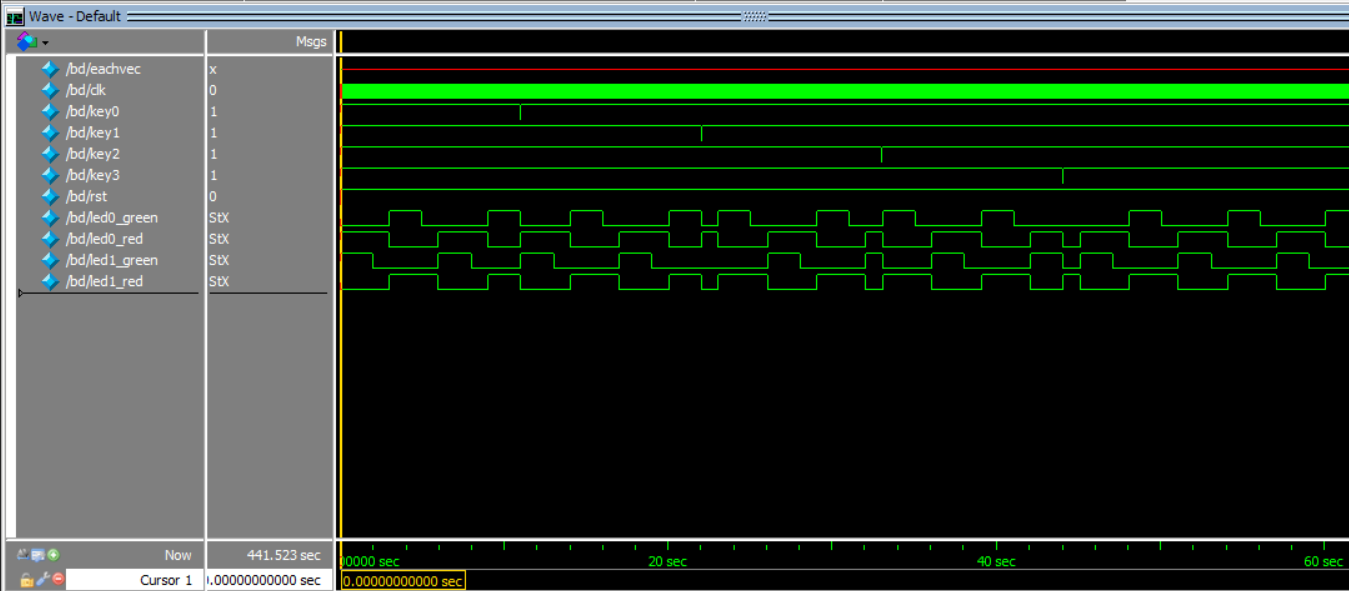
\includegraphics[width=16cm]{wave1.png}
	\caption{仿真波形图}\label{fig:wave1}
\end{figure}

\section{实验结果和分析}

通过编写代码和仿真测试后,分配好管脚,管脚分配图见附录图 \ref{fig:pin1} 所示,我们将我们的程序烧录进开发板,S0 工作状态如图 \ref{fig:work1} 所示,实验结果完全符合我们的预期,通过按按键进入对应的状态,实验不足之处在于没有添加数码管数字显示倒计时。

\begin{figure}[hbtp]
	\centering
	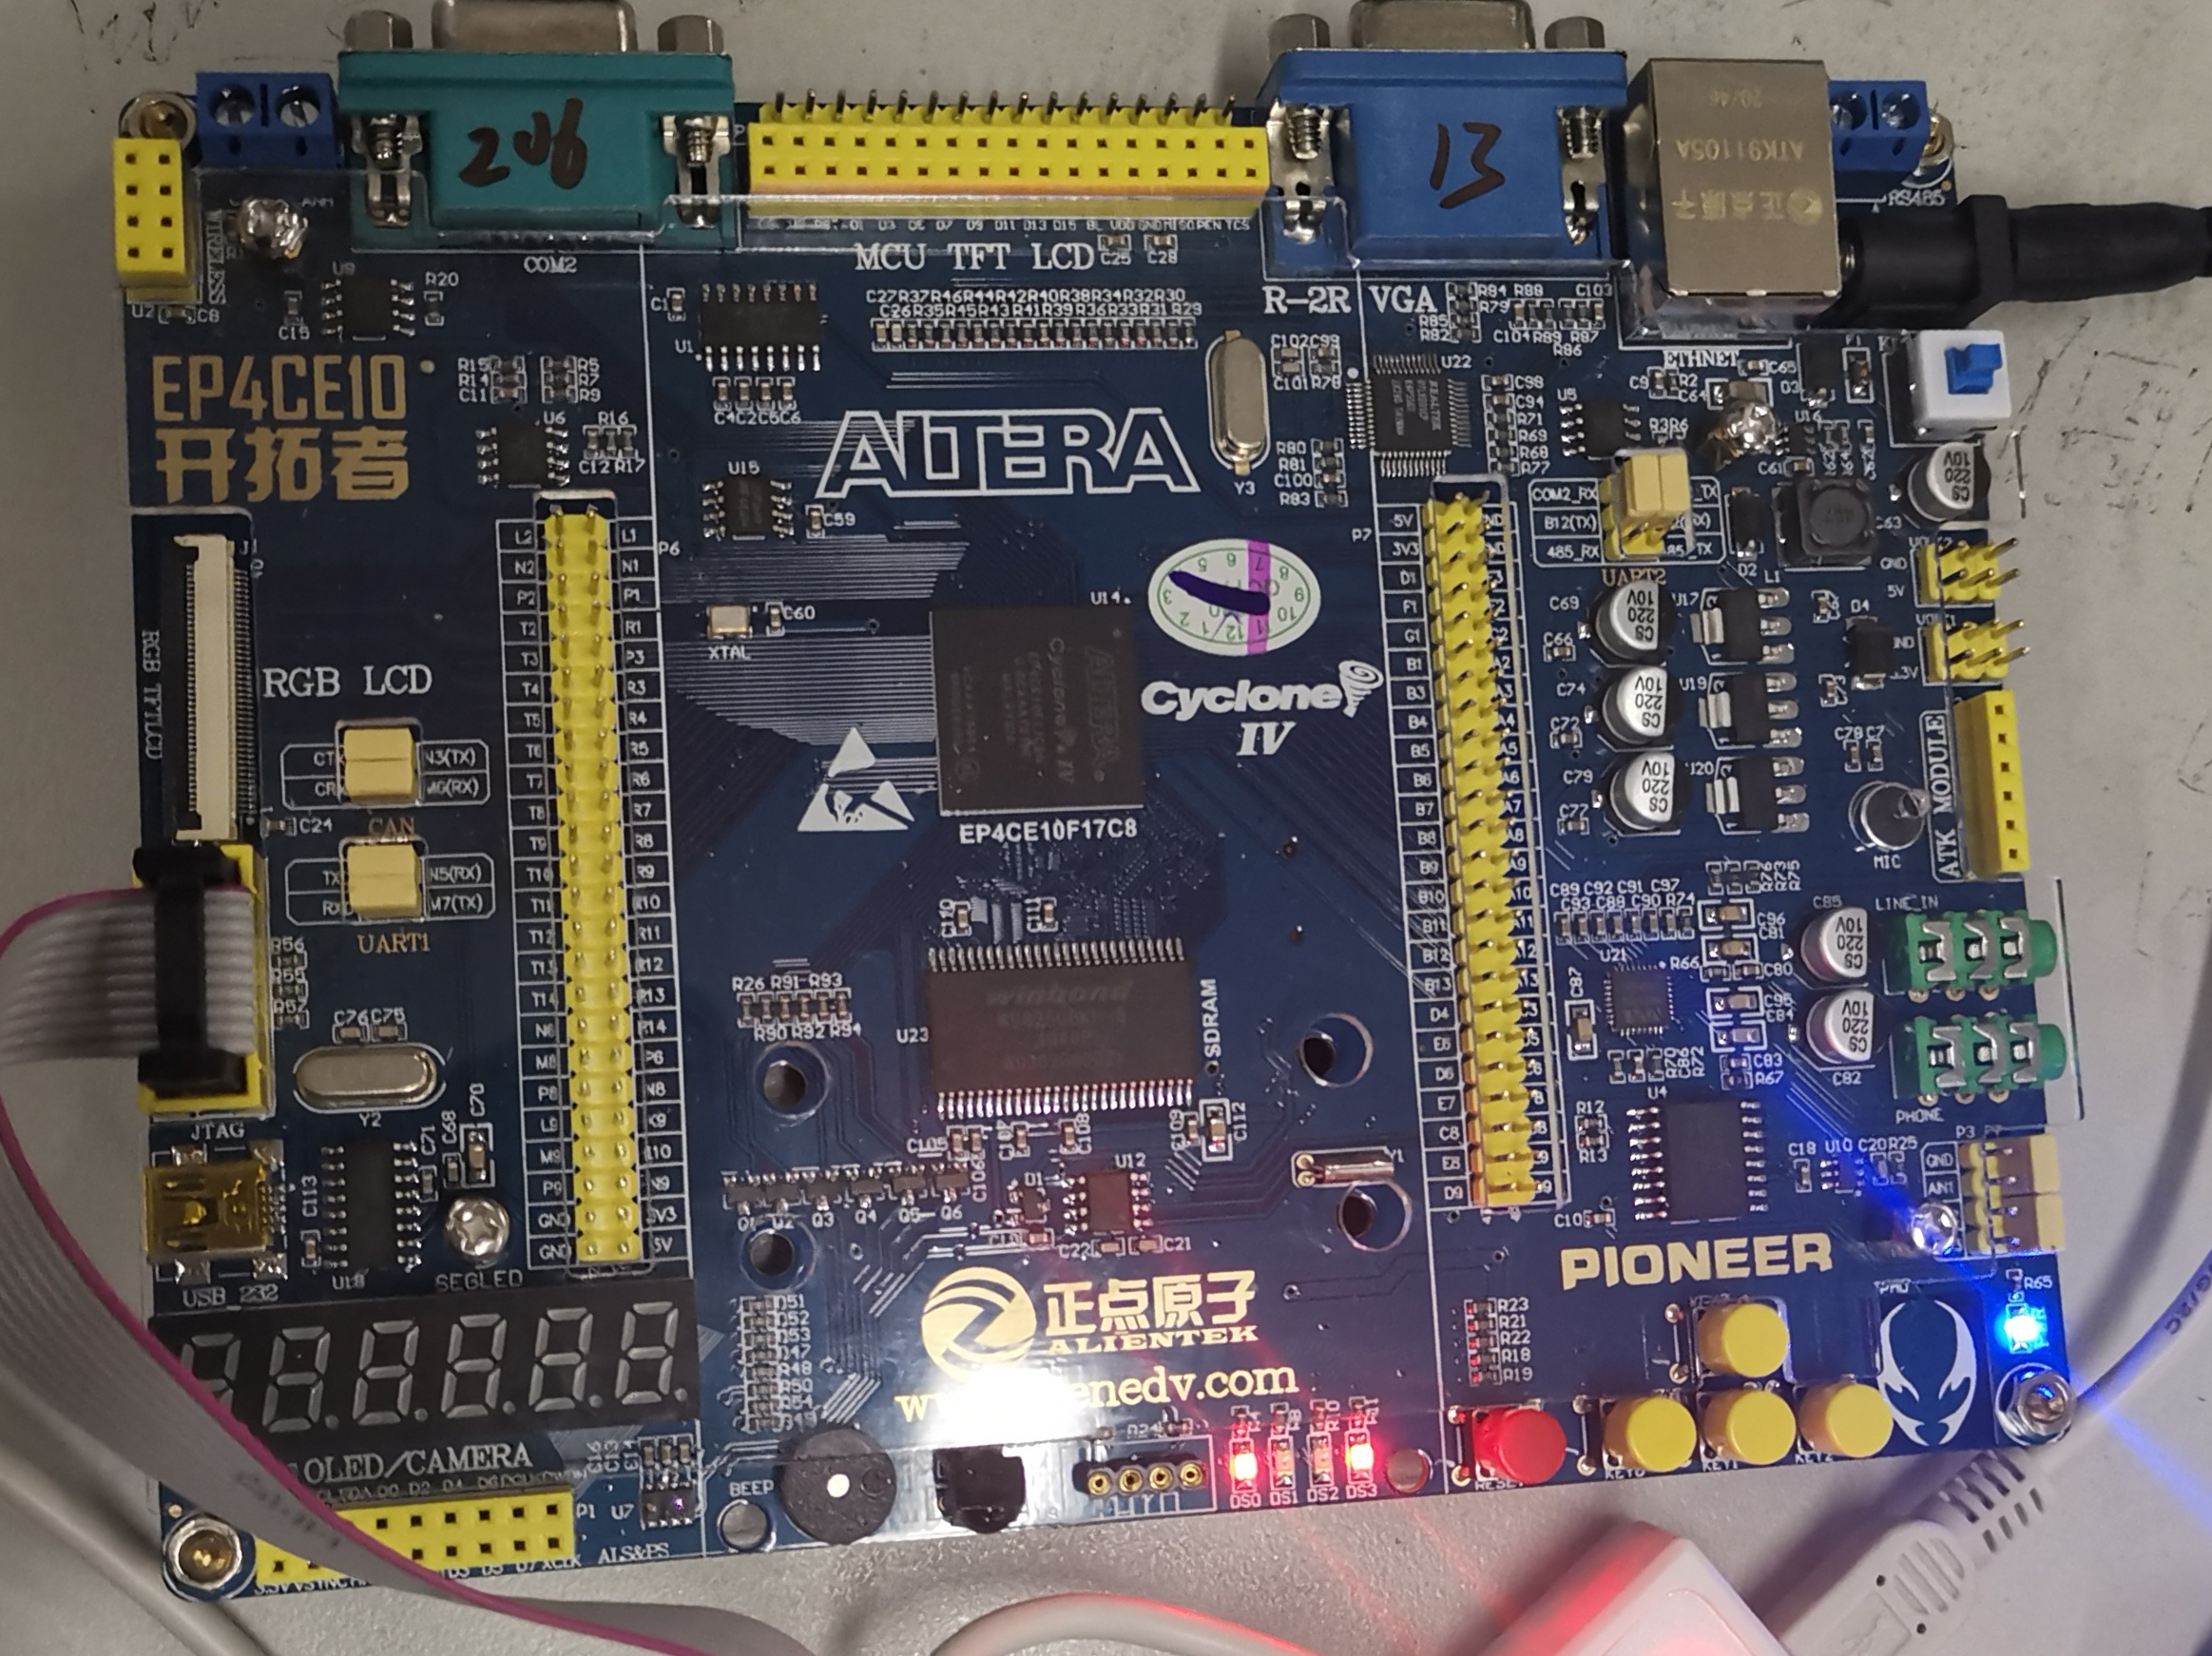
\includegraphics[width=16cm]{work1.jpg}
	\caption{S0 工作状态示意图}\label{fig:work1}
\end{figure}

\section{实验代码}

\subsection{module 1}

\begin{lstlisting}[language=Verilog]
`timescale  1ns/1ns
module  clk_div(
					clk,
					rst,
					clk_1k
					);

input clk,rst;
output clk_1k;
reg clk_1k_reg=1'b0;
reg[15:0] clk_div_cnt;

always @(posedge clk or negedge rst) 
begin
	if(rst==1'b0)
		clk_div_cnt<=0;
	else if(clk_div_cnt==24999)
		clk_div_cnt<=0;
	else
		clk_div_cnt<=clk_div_cnt+1;
end

always @(posedge clk or negedge rst) 
begin
	if(rst==1'b0)
		clk_1k_reg<=1'b0;
	else if(clk_div_cnt==24999)
		clk_1k_reg<=~clk_1k_reg;
end

assign clk_1k=clk_1k_reg;
// assign clk_1k=clk; // 仿真时上一行注释,这一行取消注释

endmodule
\end{lstlisting}

\subsection{module 2}

\begin{lstlisting}[language=Verilog]
`timescale  1ns/1ns
module  key_scan(
					clk_1k,
					rst,
					key_in,
					key_delt
					);

input clk_1k,rst;
input key_in;
output key_delt;
reg key_in_dly1,key_in_dly2;
reg[15:0] key_in_shift;
reg key_filter,key_filter_dly1;
reg[1:0] rst_cnt;

// syn key_in
always @(posedge clk_1k) 
begin
	key_in_dly1<=key_in;
	key_in_dly2<=key_in_dly1;
end

always @(posedge clk_1k) 
begin
	key_in_shift<={key_in_shift[14:0],key_in_dly2};
end

always @(posedge clk_1k or negedge rst) 
begin
	if(rst==1'b0)
		key_filter<=1'b1;
	else if(key_in_shift==0)
		key_filter<=1'b0;
	else if(key_in_shift==16'b1111111111111111)
		key_filter<=1'b1;
	else
		key_filter<=key_filter;
end

always @(posedge clk_1k) 
begin
	key_filter_dly1<=key_filter;
end

assign key_delt=(~key_filter_dly1) & key_filter;

endmodule
\end{lstlisting}

\subsection{module 3}

\begin{lstlisting}[language=Verilog]
`timescale  1ns/1ns
module  led_trans(
					clk,
					rst,
					key0,
					key1,
					key2,
					key3,
					led0_red,
					led0_green,
					led1_red,
					led1_green
					);

input clk,rst;
input key0,key1,key2,key3;
output led0_red,led0_green,led1_red,led1_green;

parameter      S0  =   4'b0000;
parameter      S1  =   4'b0001;
parameter      S2  =   4'b0011;
parameter      S3  =   4'b0111;
reg[3:0] cur_state;
reg[10:0] time_cnt;
reg led0_red_reg,led0_green_reg,led1_red_reg,led1_green_reg;
wire clk_1k;
wire key_filter0,key_filter1,key_filter2,key_filter3;


clk_div clk_div_inst(
						.clk		(clk),
						.rst		(rst),
						.clk_1k		(clk_1k)
						);

key_scan key_scan_inst0(
						.clk_1k		(clk_1k),
						.rst		(rst),
						.key_in		(key0),
						.key_delt	(key_filter0)
						);

key_scan key_scan_inst1(
						.clk_1k		(clk_1k),
						.rst		(rst),
						.key_in		(key1),
						.key_delt	(key_filter1)
						);

key_scan key_scan_inst2(
						.clk_1k		(clk_1k),
						.rst		(rst),
						.key_in		(key2),
						.key_delt	(key_filter2)
						);

key_scan key_scan_inst3(
						.clk_1k		(clk_1k),
						.rst		(rst),
						.key_in		(key3),
						.key_delt	(key_filter3)
						);

// state 
always @(posedge clk_1k or negedge rst) 
begin
	if(rst==1'b0)
		cur_state<=S0;
	else if(key_filter0==1'b1)
		cur_state<=S0;
	else if(key_filter1==1'b1)
		cur_state<=S1;
	else if(key_filter2==1'b1)
		cur_state<=S2;
	else if(key_filter3==1'b1)
		cur_state<=S3;	
	else
		case(cur_state)
		S0 : 	if(time_cnt==1999)
					cur_state<=S1;
		S1 : 	if(time_cnt==999)
					cur_state<=S2;
		S2 : 	if(time_cnt==1999)
					cur_state<=S3;
		S3 : 	if(time_cnt==999)
					cur_state<=S0;
		default : 	cur_state<=S0;
		endcase
end

// time_cnt
always @(posedge clk_1k or negedge rst) 
begin
	if(rst==1'b0)
		time_cnt<=0;
	else if(key_filter0==1'b1 | key_filter1==1'b1 | key_filter2==1'b1 | key_filter3==1'b1)
		time_cnt<=0;
	else
		case(cur_state)
		S0 : 	if(time_cnt==1999)
					time_cnt<=0;
				else
					time_cnt<=time_cnt+1;
		S1 : 	if(time_cnt==999)
					time_cnt<=0;
				else
					time_cnt<=time_cnt+1;
		S2 : 	if(time_cnt==1999)
					time_cnt<=0;
				else
					time_cnt<=time_cnt+1;
		S3 : 	if(time_cnt==999)
					time_cnt<=0;
				else
					time_cnt<=time_cnt+1;
		default : 	time_cnt<=0;
		endcase
end

// led0_red
always @(posedge clk_1k) 
begin
	case(cur_state)
	S0 : 	led0_red_reg<=1'b1;
	S1 : 	led0_red_reg<=1'b1;
	S2 : 	led0_red_reg<=1'b0;
	S3 : 	led0_red_reg<=1'b0;
	default : 	led0_red_reg<=1'b0;
	endcase
end

// led0_green
always @(posedge clk_1k) 
begin
	case(cur_state)
	S0 : 	led0_green_reg<=1'b0;
	S1 : 	led0_green_reg<=1'b0;
	S2 : 	led0_green_reg<=1'b1;
	S3 : 	led0_green_reg<=1'b0;
	default : 	led0_green_reg<=1'b0;
	endcase
end

// led1_red
always @(posedge clk_1k) 
begin
	case(cur_state)
	S0 : 	led1_red_reg<=1'b0;
	S1 : 	led1_red_reg<=1'b0;
	S2 : 	led1_red_reg<=1'b1;
	S3 : 	led1_red_reg<=1'b1;
	default : 	led1_red_reg<=1'b0;
	endcase
end

// led1_green
always @(posedge clk_1k) 
begin
	case(cur_state)
	S0 : 	led1_green_reg<=1'b1;
	S1 : 	led1_green_reg<=1'b0;
	S2 : 	led1_green_reg<=1'b0;
	S3 : 	led1_green_reg<=1'b0;
	default : 	led1_green_reg<=1'b0;
	endcase
end

assign led0_red=led0_red_reg;
assign led0_green=led0_green_reg;
assign led1_red=led1_red_reg;
assign led1_green=led1_green_reg;

endmodule
\end{lstlisting}

\subsection{仿真测试代码}

\begin{lstlisting}[language=Verilog]
// Copyright (C) 1991-2013 Altera Corporation
// Your use of Altera Corporation's design tools, logic functions 
// and other software and tools, and its AMPP partner logic 
// functions, and any output files from any of the foregoing 
// (including device programming or simulation files), and any 
// associated documentation or information are expressly subject 
// to the terms and conditions of the Altera Program License 
// Subscription Agreement, Altera MegaCore Function License 
// Agreement, or other applicable license agreement, including, 
// without limitation, that your use is for the sole purpose of 
// programming logic devices manufactured by Altera and sold by 
// Altera or its authorized distributors.  Please refer to the 
// applicable agreement for further details.

// ***********************************************************************
// This file contains a Verilog test bench template that is freely editable to  
// suit user's needs .Comments are provided in each section to help the user    
// fill out necessary details.                                                  
// ***********************************************************************
// Generated on "10/30/2021 10:55:37"

// Verilog Test Bench template for design : led_trans
// 
// Simulation tool : ModelSim-Altera (Verilog)
// 

`timescale 100 us/ 100 us
module bd();
// constants                                           
// general purpose registers
reg eachvec;
// test vector input registers
reg clk;
reg key0;
reg key1;
reg key2;
reg key3;
reg rst;
// wires                                               
wire led0_green;
wire led0_red;
wire led1_green;
wire led1_red;

// assign statements (if any)                          
led_trans i1 (
// port map - connection between master ports and signals/registers   
	.clk(clk),
	.key0(key0),
	.key1(key1),
	.key2(key2),
	.key3(key3),
	.led0_green(led0_green),
	.led0_red(led0_red),
	.led1_green(led1_green),
	.led1_red(led1_red),
	.rst(rst)
);
initial                                                
begin                                             
#0                         
clk=1'b0;
rst=1'b0;
key0=1'b1;
key1=1'b1;
key2=1'b1;
key3=1'b1;
#1
rst=1'b1;

#110000
key0=1'b0;
#200
key0=1'b1;

#110000
key1=1'b0;
#200
key1=1'b1;

#110000
key2=1'b0;
#200
key2=1'b1;

#110000
key3=1'b0;
#200
key3=1'b1;

//#300000000
//$stop;                                                
// --> end                                             
$display("Running testbench");                       
end                                                    
always   
#5
clk=~clk;                
begin                                                  
// code executes for every event on sensitivity list   
// insert code here --> begin                          

// --> 
end                                               
endmodule
\end{lstlisting}

% % 参考文献,此处以 MLA 引用格式为例

%\begin{thebibliography}{9}
%\end{thebibliography}

% % \includepdf[pages={1,2}]{Memo.pdf} 
% 可以直接导入pdf页面
\newpage

\begin{appendices}  % 附录环境

\section{管脚分配}

\begin{figure}[hbtp]
	\centering
	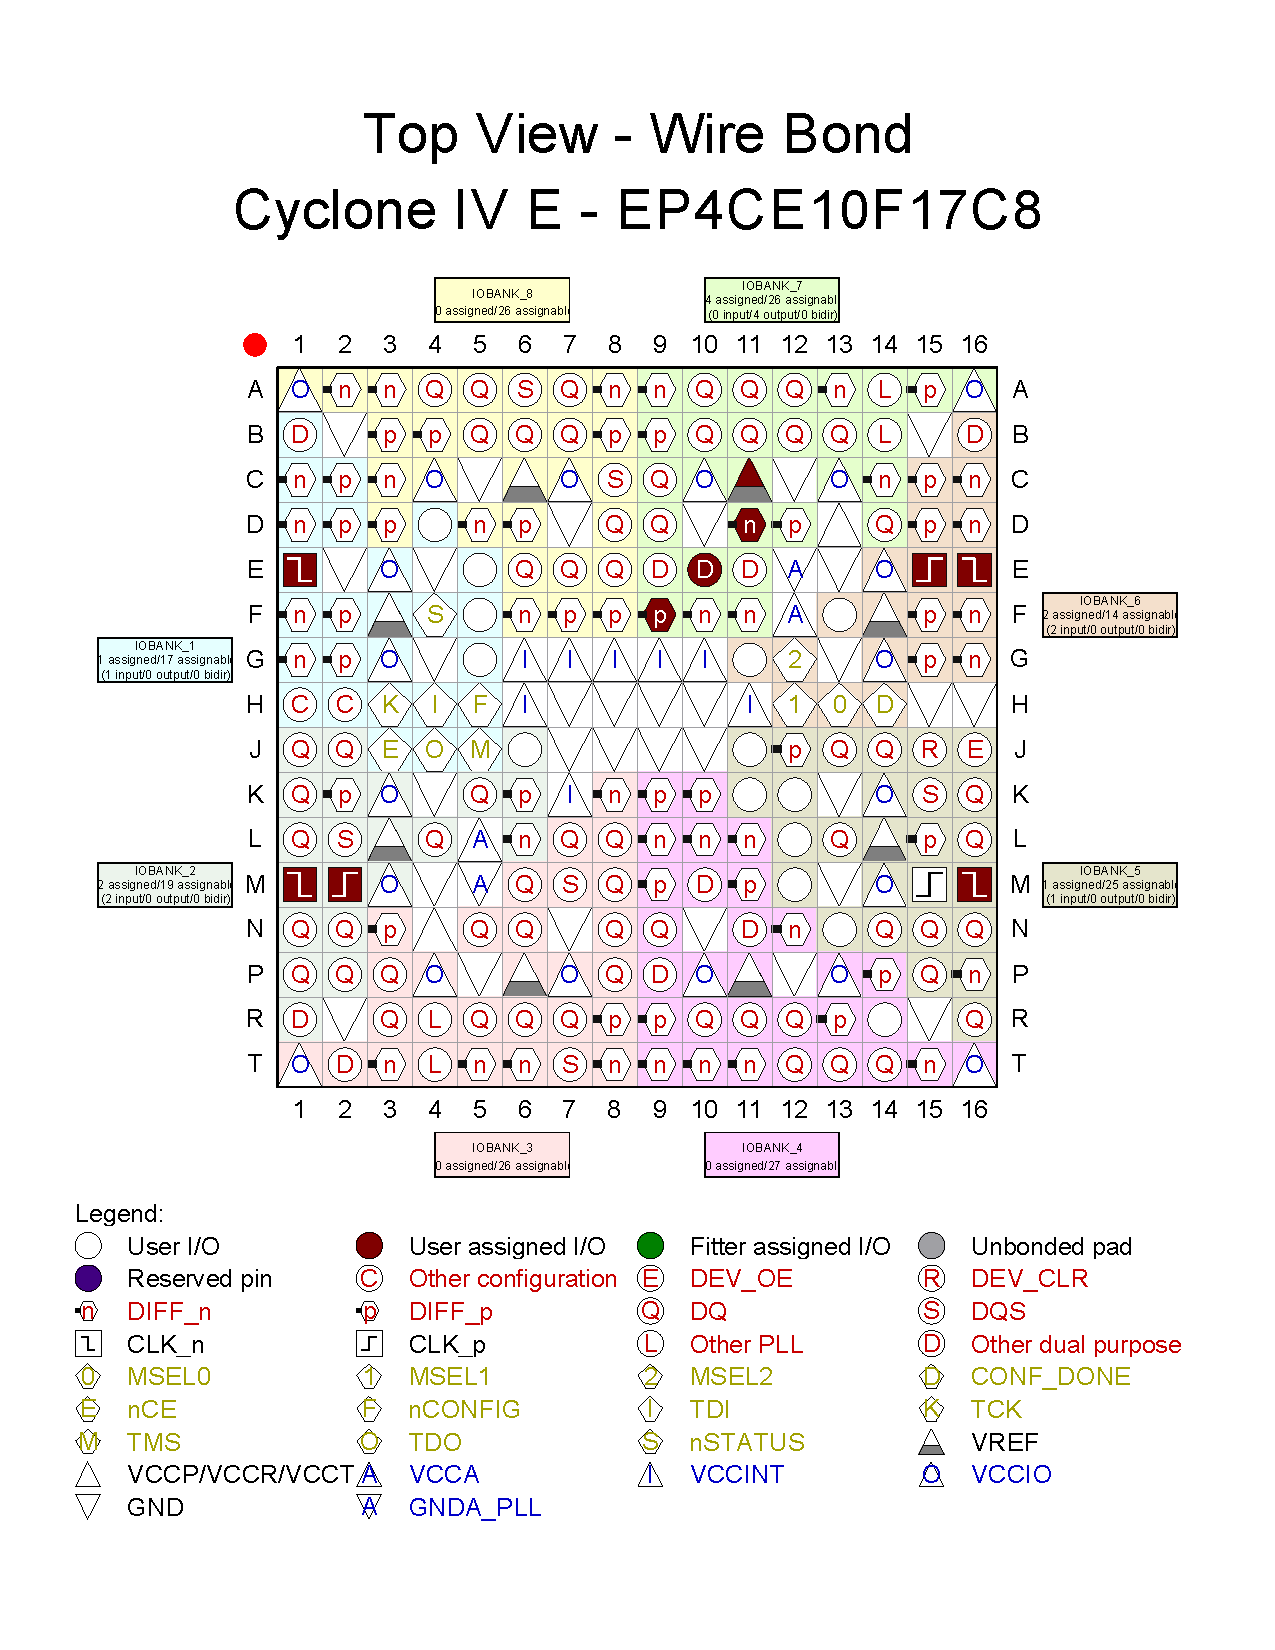
\includegraphics[width=15.5cm]{pin1.pdf}
	\caption{管脚分配图}\label{fig:pin1}
\end{figure}

\end{appendices}
\end{document}  % 结束